
%(BEGIN_QUESTION)
% Copyright 2006, Tony R. Kuphaldt, released under the Creative Commons Attribution License (v 1.0)
% This means you may do almost anything with this work of mine, so long as you give me proper credit

Anta at vi utstyrer en elektrisk stekeovn med følgende proporsjonalreguleringssystem. En {\it instrumenteringsforsterker} utgjør kjernen i dette reguleringssystemet, og gir ut en spenning proporsjonal med spenningsforskjellen mellom den ikke-inverterende og den inverterende inngangen. En ekstern motstand setter differensialforsterkningen til forsterkeren:

$$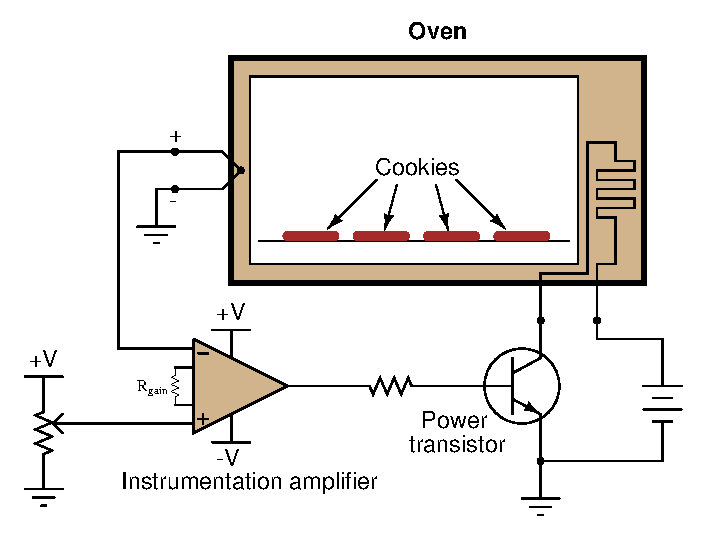
\includegraphics[width=15.5cm]{i01456x03.eps}$$

Når vi måler temperatur over tid med en {\it skriver}, ser vi denne grafen for ovnstemperatur over tid:

$$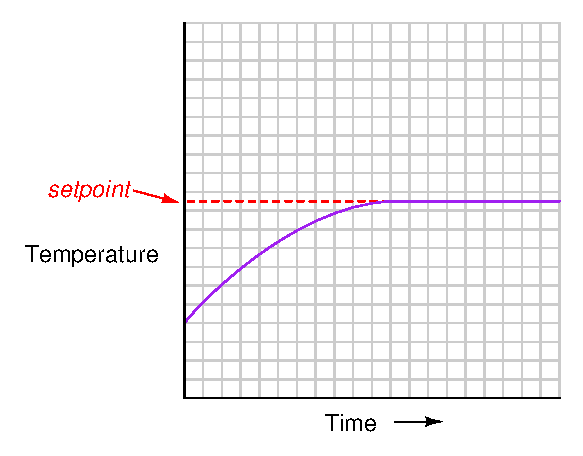
\includegraphics[width=15.5cm]{i01456x01.eps}$$

Temperaturen stiger langsomt fra omgivelsestemperatur mot settpunkt, og nærmer seg settpunkt asymptotisk (langsommere jo nærmere den kommer), helt til den til slutt når målet.

At prosessvariabelen når settpunkt nøyaktig er selvsagt ett av målene med et reguleringssystem. Men det er ikke det eneste målet. Ideelt sett vil vi at prosessvariabelen skal nå settpunktet {\it så raskt som mulig}. Hvordan kan proporsjonalreguleringen endres for å øke responstiden i reguleringssystemet i forhold til det som er vist her? Hva må endres eller justeres for at proporsjonalreguleringen skal reagere raskere for å nå settpunkt?

Hint: analyser problemet ut fra hvordan systemet oppfører seg nå. Hva gjør et proporsjonalreguleringssystem feil hvis prosessvariabelen nærmer seg settpunkt så sakte? Tenk deg at du sitter i en bil med en fører som korrigerer kjørefeltposisjon eller hastighet svært tregt. Hva gjør en god sjåfør annerledes enn en treg sjåfør?
 
\underbar{file i01456}
%(END_QUESTION)





%(BEGIN_ANSWER)

Problemet med dette reguleringssystemet er at utgangen ikke reagerer aggressivt nok på endringer i inngangen. Det vi trenger, er en regulator som metter (100\% utgangssignal til transistoren som styrer varmeelementet) så lenge temperaturen ligger betydelig under settpunkt, og som først begynner å ``strupe'' når vi nærmer oss settpunkt.

Jeg lar deg finne ut hva som må endres i denne kretsen for å forbedre reguleringsoppførselen!

%(END_ANSWER)





%(BEGIN_NOTES)

For å forbedre responstiden til dette proporsjonalreguleringssystemet må vi øke spenningsforsterkningen til differensialforsterkeren. Hvis vi gjør denne endringen i reguleringskretsen, vil vi se en forbedret reguleringsrespons som kan se omtrent slik ut:

$$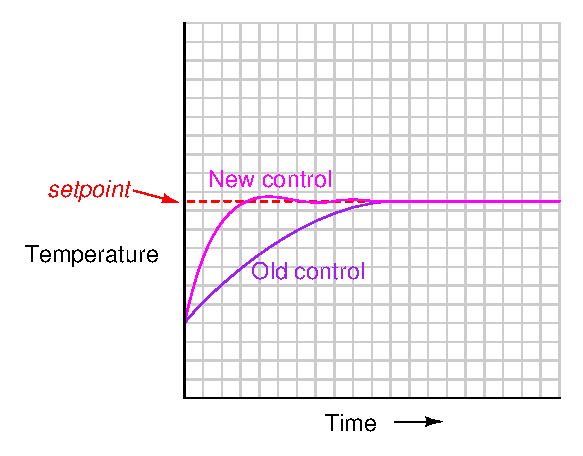
\includegraphics[width=15.5cm]{i01456x02.eps}$$

\vskip 20pt \vbox{\hrule \hbox{\strut \vrule{} {\bf Virtuell feilsøking} \vrule} \hrule}

Dette spørsmålet egner seg godt som en ``Virtuell feilsøking''-øvelse. Når du presenterer diagrammet for studentene, forestiller du deg først en bestemt feil i systemet. Deretter presenterer du ett eller flere symptomer på denne feilen (noe en operatør eller annen bruker kan observere). Studentene foreslår så ulike diagnostiske tester for å identifisere feilens natur og plassering, slik teknikere ville gjort i praktisk feilsøking. Din oppgave er å fortelle hva resultatet ville blitt for hver foreslått test, og dokumentere resultatene slik at alle studentene kan se dem.

Under og etter øvelsen er det nyttig å stille oppfølgingsspørsmål som:

\begin{itemize}
\item{} Hva forteller resultatet av den siste diagnostiske testen deg om feilen?
\item{} Anta at resultatene av den siste diagnostiske testen var annerledes. Hva ville det resultatet fortalt deg om feilen?
\item{} Er den siste diagnostiske testen den beste vi kunne gjort?
\item{} Hva ville vært ideell testrekkefølge for å diagnostisere problemet i færrest mulig trinn?
\end{itemize}


%INDEX% Control, proportional: controller gain

%(END_NOTES)

